% LaTeX-Vorlage zur Erstellung einer Abschlussarbeit in der Fakultät Elektrotechnik, Medien und Informatik an der OTH Amberg-Weiden
% Diese Vorlage entstand im Rahmen des Kurses "LaTeX fürs Studium"
% Aktuelle Version: v0.03bacsem
% Stand: 18.04.2020
%
% Changelog:
%
% v0.03bacsem-us: 28.04.2020, Grafikpfad und Bibliographiemanagement 
%                             via bibtex hinzugefügt
% Grafikpfad für das graphicx-Paket:
%   \graphicspath{{images/}} % hinter \usepackage{graphicx}
% Literaturverzeichnis nach DIN:          
%   \usepackage[square,numbers,sort]{natbib} 
% Literaturverzeichnis am Ende:
%   \bibliographystyle{natdin}
%   \bibliography{literatur}
% 
% v0.02: 06.08.2015, Anpassung der Vorlage:
% + Persönliche Informationen (Vorname, Name, Titel usw.) werden direkt in die PDF-Dokumenteinstellungen übernommen
% + Korrektur der Verlinkung von Abbildungs- und Tabellenverzeichnis aus dem Inhaltsverzeichnis (phantomsection) bzw. deren Seitenzahl
%   Besten Dank für diesen Hinweis an Jan-Olaf Becker
% + Anpassung des Namens der Fakultät nach deren Umbenennung
%
% v0.01: 14.03.2012, Erstellung der Vorlage
% oneside: legt Seitennummerierung in die Mitte -> einseitiger Druck
% twoside: legt Seitennummerierung abh. von Seite an rechten/linken Rand -> vorder-/rueckseite Druck
\documentclass[12pt,oneside]{report}
\usepackage[T1]{fontenc}		% Einstellungen fuer Umlaute usw.
\usepackage[utf8x]{inputenc}
\usepackage[ngerman]{babel}

\usepackage{parskip}			% Einstellungen fuer Absaetze: Abstand statt Einrueckung

\usepackage[a4paper,			% Papierformat A4
	    left=2.0cm,				% linker Rand
	    right=2.0cm,			% rechter Rand
	    top=2.0cm,				% oberer Rand
	    bottom=2.0cm,			% unter Rand
	    marginparsep=5mm,		% Abstand der Randnotizen
	    marginparwidth=10mm, 	% Breite der Randnotizen
	    headheight=7mm,			% Hoehe der Kopfzeile
	    headsep=1.2cm,			% Abstand der Kopfzeile
	    footskip=1.5cm,			% Abstand der Fusszeile
	    includeheadfoot]{geometry}

\usepackage{fancyhdr}						% Konfiguration von Kopf- und Fusszeilen
\pagestyle{fancy}							% Seitenstil 'fancy'
\fancyhf{}									% vorhandene Einstellungen loeschen
\setlength{\headwidth}{\textwidth}			% Kopf- und Fusszeile so breit wie der Haupttext
\fancyfoot[R]{\thepage} 					% Festlegung des Seitenstils: Seitenzahlen in der Fusszeile rechts
\fancyfoot[L]{\leftmark}					% Kapitelnr. und -Bezeichnung in der Fusszeile links
\fancyhead[R]{\IhreArbeit}					% "Bachelorarbeit" in der Kopfzeile rechts
\fancyhead[L]{\IhrVorname\ \IhrNachname}	% Vorname und Name in der Kopfzeile links
\renewcommand{\chaptermark}[1]{			% Definition der Ausgabe des Kapitels
  \markboth{Kapitel \thechapter. #1}{}}
\renewcommand{\headrulewidth}{0.5pt}		% Trennlinie zwischen Kopfzeile und Haupttext
\renewcommand{\footrulewidth}{0.5pt}		% Trennlinie zwischen Haupttext und Fusszeile
\fancypagestyle{plain}{					% Anpassung des Seitenstils 'plain' bei Beginn neuer Kapitel
  \fancyhf{}								% Vorbelegung loeschen
  \fancyfoot[C]{\thepage}					% Seitenzeilen in der Fusszeile mittig
  \fancyhead[R]{\IhreArbeit}				% "Bachelorarbeit" in der Kopfzeile rechts
  \fancyhead[L]{\IhrVorname\ \IhrNachname}	% Vorname und Name in der Kopfzeile links
}

%\usepackage{amsmath}			% Pakete fuer den Mathematikmodus
%\usepackage{amssymb}
\usepackage[intlimits]{empheq}

\usepackage[sc]{mathpazo}		% Schriftart Palatino fuer Haupttext und Mathematikmodus
\usepackage{pifont}				% zusaetzliche Symbole

\usepackage{setspace}
\setstretch{1.25}

\usepackage[format=hang,		% Einstellung fuer Bildunterschriften
            font={footnotesize},
            labelfont={bf},
            margin=1cm,
            aboveskip=5pt,
            position=bottom]{caption}

\usepackage{graphicx}	   % Einbinden von Grafiken (jpg, png, pdf, ...)
\graphicspath{{images/}}   % Suchpfad für Grafikdateien

\usepackage[svgnames,table,hyperref]{xcolor} 	% Verwendung von Farben
\usepackage{tikz}								% Erstellen von Grafiken
\usetikzlibrary{positioning,arrows,plotmarks} % TikZ-Bibliotheken
%\usepackage{pgfplots}                           % Darstellung von Plots, Funktionen, Graphen usw.

%
% Weitere Pakete
%
\usepackage{listings}			% Darstellung von Quellcode
\definecolor{mygreen}{rgb}{0,0.6,0}
\definecolor{myblue}{rgb}{0.0,0.0,1.0}
\definecolor{myred}{rgb}{1.0,0.3,0.0}

\DeclareMathOperator{\arctantwo}{arctan2}

\usepackage{leftidx}

\lstset{language = Python,
	numbers = none,
	basicstyle = \small\ttfamily,
	keywordstyle = \color{myblue},
	commentstyle = \color{mygreen},
	stringstyle = \color{myred},
	columns = flexible,
	showstringspaces = false,
	frame = single,
	morekeywords={as, family}
}
\usepackage{float}
\usepackage[square,numbers,sort]{natbib} % Referenzen
%
%\usepackage[european, siunitx]{circuitikz}	% Darstellung von Schaltungen
%
%\usepackage{enumerate}			% Formatierung nummerierter Listen

\usepackage{microtype,relsize}					% Wird verwendet, um Nachnamen auf Titelseite gesperrt darzustellen
\newcommand*{\Sperren}[1]{\textls*[100]{#1}}

% 
% Persoenliche Angaben
% 
\newcommand*{\IhrVorname}{André}
\newcommand*{\IhrNachname}{Kestler}
\newcommand*{\IhrStudiengang}{Künstliche Intelligenz}
% Bachelorarbeit, Masterarbeit, Studienarbeit
\newcommand*{\IhreArbeit}{Studienarbeit AR/VR}
\newcommand*{\IhrTitelDE}{Der Igel Simulator}
% \newcommand*{\IhrTitelEN}{Title of the study work}
\newcommand*{\IhrBearbeitungszeitraumVON}{01. Dezember 2021}
\newcommand*{\IhrBearbeitungszeitraumBIS}{02. Februar 2022}
\newcommand*{\IhrErstpruefer}{Prof. Dr.-Ing. Gerald Pirkl}
% \newcommand*{\IhrZweitpruefer}{Prof. Dr.-Ing. Franz Klug}
% \newcommand*{\IhreFirma}{OTH Amberg-Weiden}
% \newcommand*{\IhrFirmenbetreuer}{Prof. Dr.-Ing. Matthias Wenk}
\newcommand*{\IhreZusammenfassung}{Zusammenfassung}

\newcommand*{\IhreSchluesselwoerter}{Schlüsselwortliste}

\newcommand*{\IhrAbstract}{Abstract}



\usepackage[bookmarks, raiselinks, pageanchor, % PDF-Einstellungen
            hyperindex, colorlinks,
            citecolor=black, linkcolor=black,
            urlcolor=black, filecolor=black,
            menucolor=black]{hyperref}
\hypersetup{pdftitle={\IhrTitelDE},%
            pdfauthor={\IhrVorname\ \IhrNachname},%
            pdfsubject={\IhreArbeit},%
            pdfkeywords={\IhreSchluesselwoerter}}

%
% Beginn des Textteils
%
\begin{document}
    \pagenumbering{roman}
  \thispagestyle{empty}
  \begin{center}
    \Large
    Ostbayerische Technische Hochschule Amberg-Weiden\\
    Fakultät Elektrotechnik, Medien und Informatik\\[1cm]
    Studiengang \IhrStudiengang\\[1cm]
    \textbf{\IhreArbeit}\\[1cm]
    von\\[1cm]
    \IhrVorname\ \Sperren{\textbf{\IhrNachname}}\\[1cm]
    \textbf{\IhrTitelDE}\\[1cm]
%    \IhrTitelE
  \end{center}
  \vspace*{2.5cm}
  \begin{tabbing}
    \underbar{Bearbeitungszeitraum:}\qquad\= von\qquad\=\IhrBearbeitungszeitraumVON\\
                                          \> bis      \>\IhrBearbeitungszeitraumBIS
  \end{tabbing}
  \vspace*{1cm}
  \underbar{1. Prüfer:}\qquad\IhrErstpruefer\par 
 % \underbar{2. Prüfer:}\qquad\IhrZweitpruefer
    \tableofcontents
    \thispagestyle{empty}
 	\newpage
  
% ----------------------------------------------------------------------  
  
%  \chapter*{Symbole, Formelzeichen und Einheiten}
 % \begin{tabular}{ll}
 % 	%$I$ & Einheitsmatrix\\
 % 	%GB     & Gigabyte ($10^9$ Bytes)\\
 % \end{tabular}
 % \newpage
  
% ----------------------------------------------------------------------  
  \chapter*{Abkürzungsverzeichnis}
    \begin{tabular}{ll}
    	%KI	& Künstliche Intelligenz\\
    	%TCP & Tool Center Point\\  		
    	AR & Augmented Reality\\
    	VR & Virtual Reality\\
    	MR & Mixed Reality
  	\end{tabular}

  \newpage
  \pagenumbering{arabic}
  % Kapitel einfügen
  \chapter{Einleitung}

\section{Aufgabenstellung}
Im Rahmen des Studiengangs Ausgewählte Themen AR/VR soll ein Projekt im Themenbereich Augmented Reality (AR), Virtual Reality (VR) oder Mixed Reality (MR) bearbeitet werden. Die Bearbeitung des eigens ausgesuchten Projekts soll in einer Gruppe erfolgen. Die Gruppe für dieses Projekt besteht aus folgenden Personen: Johannes Horst, Saniye Ogul, Stefanie Hofmann, Magdalena Bienefeld und mir (André Kestler). Als Projekt wurde ein Igel Simulator als VR-Spiel entworfen und programmiert. Mit der VR-Brille Oculus Quest kann das Spiel an einem Computer mithilfe des Link-Kabels gespielt werden. 


\section{Projektmanagement}
\subsection{GitHub}
Zur Versionsverwaltung des Projekts wurde GitHub verwendet. Dort hat Johannes Horst ein Repository für das Projekt angelegt und jeder Teilnehmer hat seine Arbeiten dort einchecken können. Außerdem ist durch dieses Tool jeder auf dem aktuellsten Softwarestand und Fehler können einfach überblickt werden. \cite{GitHub}


\subsection{Trello}
Bei Trello handelt es sich um einen Onlinedienst, der ein Projekt bei der Verwaltung und Verteilung von Aufgaben unterstützt. Durch ihn lassen sich Arbeitsboards anlegen und in diesem Listen für bestimmte Themengebiete. In den Listen können Karten für die zu bearbeitenden Aufgaben erstellt werden und Benutzer zugeordnet werden. Der Vorteil ist, dass man immer einen Überblick über die Aufgaben hat und zum Ende des Projekts eine Übersicht über die bearbeiteten Themen hat. \cite{Trello}

\subsection{Discord}
Zur Absprache und Klärung von Problemen wurde auf das Kommunikationstool Discord zurückgegriffen. Darin wurden wöchentlich Meetings angesetzt, um den Zwischenstand und die Aufgabenverteilung festzulegen.

\subsection{Unity}
Für das zu bearbeitende Thema hat sich meine Gruppe für, die in der Vorlesung kennengelernte Spielentwicklungsumgebung, Unity entschieden. Die Anwendung wurde mit der Unity Version 2020.3.20f1 entwickelt.  \cite{Unity}


  % Hauptteil
  \chapter{Spielvorstellung}
\section{Spielmechanik}
%Was soll passieren
%Was ist Sinn hinter dem Spiel
%Karte zu beginn -> Karte des Spiels am Ende -> Evolution der Entwicklung
Die Idee meiner Gruppe, war es ein Spiel zu entwerfen, welches zusätzlich zu den unterhaltenden Faktor auch noch einen lehrenden Einfluss besitzt. In einer virtuellen Welt spielt der Spieler einen Igel in First-Person. Dazu kann sich der Spieler mit den Controllern auf der Karte, welche in \autoref{fig:map} dargestellt ist, fortbewegen. Im Laufe des Spiels lernt der Anwender wissenswertes über Igel und muss sein Wissen bei den verschiedenen Stationen auf die Probe stellen. Das erfolgreiche Bearbeiten der Stationen ist nötig, da man als Errungenschaft jeweils ein Blatt erhält. Wenn alle Blätter gesammelt wurden, wird das Spiel im Haus der Igelfamilie beendet.

\begin{figure}[H]
	\centering
	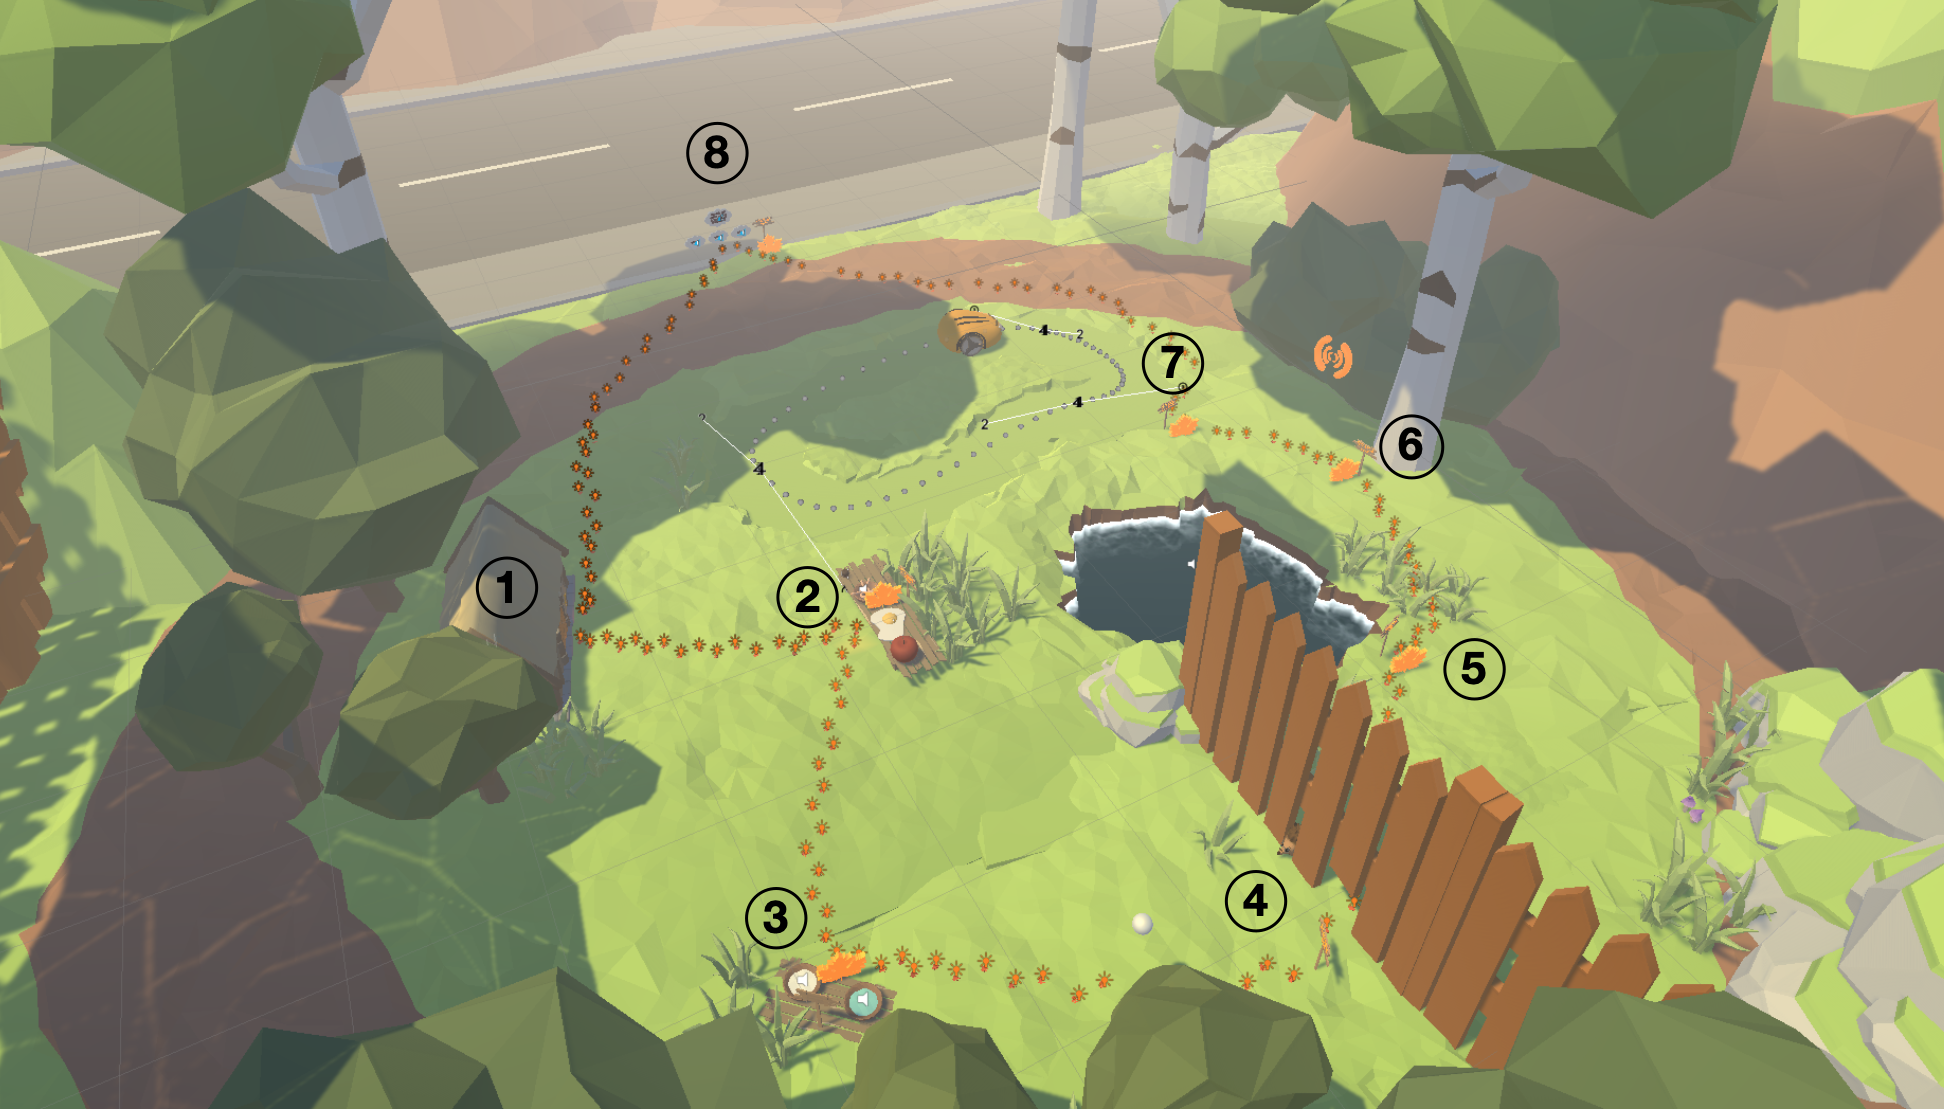
\includegraphics[width=0.675\linewidth]{map.png}
	\caption[Übersicht über die Spielkarte]{Übersicht über die Spielkarte 1: Tutorial, 2: Essen, 3: Trinken, 4: Zaun, 5: Teich, 6: Feind, 7: Rasenmäher, 8: Straße. Quelle: Eigene Aufnahme}
	\label{fig:map}
\end{figure}
 
Zur Steuerung wurde eine Kombination aus Teleportation und Fortbewegung mit den Joysticks der Controller gewählt. Es wurde keine reine physische Fortbewegung implementiert, da die Karte des Spiels sonst auf die jeweilige begehbare reale Umgebung angepasst werden muss. Damit ist das Spiel auch unabhängig der räumlichen Möglichkeiten spielbar.


\section{Immersion}
Ein Spiel wird als immersiv bezeichnet, wenn der Spieler vollständig in die fiktive Welt eintaucht und dabei die Wahrnehmungen der realen Umgebung sinken oder gänzlich verschwinden. Dies wurde in dem Spiel mithilfe der Größe der modellierten Umgebung versucht zu erreichen. Da ein Igel relativ klein ist, wurde die Welt mit seinen Gegenständen dementsprechend größer modelliert. Dieser Sachverhalt ist in \autoref{fig:big_objects} zu sehen. Für ein schöneres Spielgefühl sind zudem noch Audiobestandteile eingefügt, welche für ein besseres Ambiente sorgen. So sind an der Straße die Autos oder bei der Station des Rasenmähers dieser zu hören.

\begin{figure}[H]
	\centering
	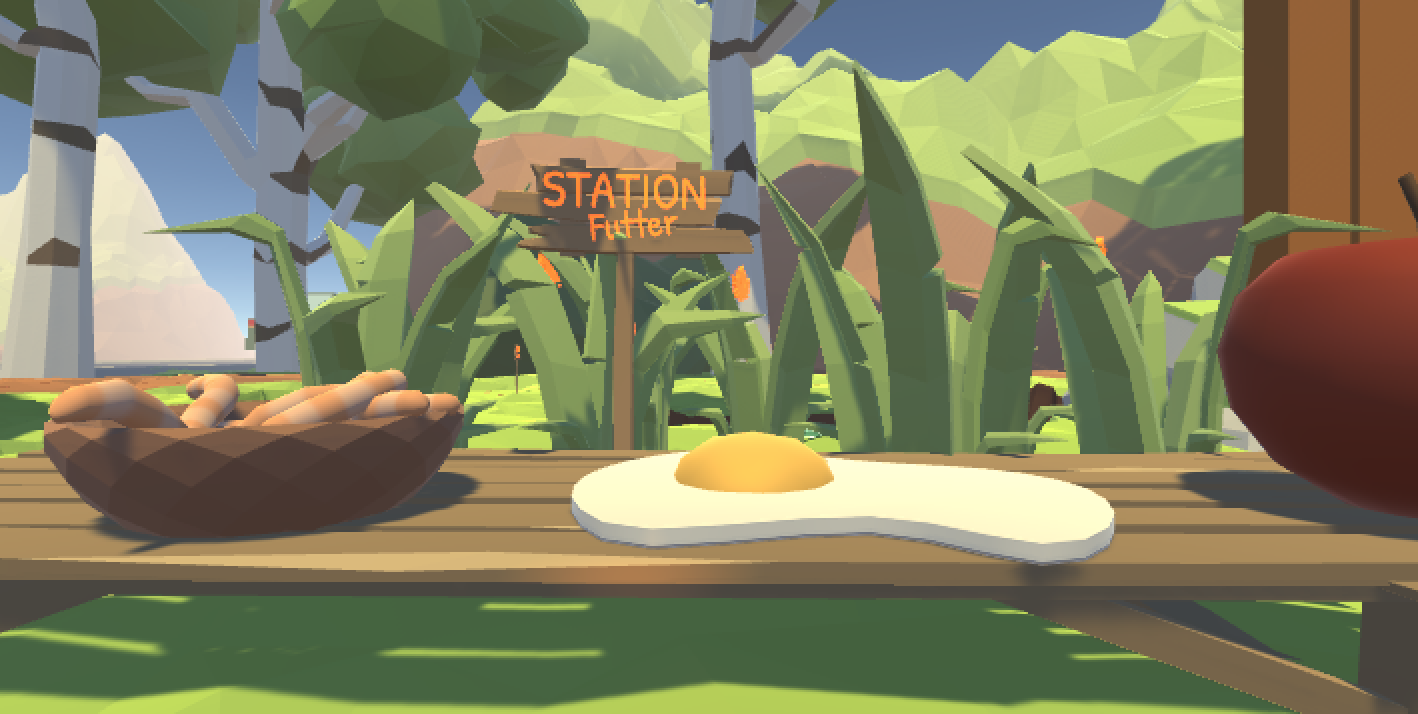
\includegraphics[width=0.55\linewidth]{big_objects.png}
	\caption[Darstellung der Größenunterschiede]{Darstellung der Größenunterschiede. Quelle: Eigene Aufnahme}
	\label{fig:big_objects}
\end{figure}

Es sei aber zu erwähnen, dass durch die Wahl der Fortbewegungsmethode und der Low-Poly Grafik der Effekt der Immersion gemindert wird.

  \chapter{Entwicklung}
\section{Igel Informationen}
Da das Spiel einen Einblick in die Lebensweise eines Igels geben soll, mussten im ersten Schritt die dazu nötigen Informationen eingeholt werden. Dazu wurde zum einen im Internet danach gesucht und Magdalena Bienefeld hatte sich mit Jana Zwanziger aus Führt getroffen, die eine Pflegeeinrichtung für Igel führt. Dadurch konnten Informationen aus erster Hand gesammelt werden. \cite{Igelrettung} 

Um Igel zu unterstützen, soll man ihnen als Nahrungsmöglichkeit keine Milch zur Verfügung stellen, sondern Wasser. Igel können Milch nicht verarbeiten, da sie Laktoseintolerant sind. Am liebsten Fressen sie Käferlarven, Raupen oder Regenwürmer. Zur Unterstützung der  Nahrungsfindung kann der Mensch ihnen Katzenfutter oder Eier zur Verfügung stellen. Auf keinen Fall dürfen sie Äpfel, Nüsse oder andere Speisereste erhalten. 

Neben den natürlichen Fressfeinden wie dem Dachs, dem Uhu oder dem Fuchs sind in den letzten Jahren durch den technologischen Fortschritt die Straßen mit den Autos und vor allem die Rasenmäherroboter hinzugekommen, da diese meistens auch dann in den Gärten fahren, wenn Igel auf ihren Streifzügen sind. Durch den Verlust von naturnahen Gärten verlieren Igel immer weiter ihren Lebensraum. 

Igel halten auch einen Winterschlaf, da sie in den Monaten zu wenig Nahrung finden würden. Abhängig von der Witterung suchen sie sich gegen November einen Unterschlupf. Während des Schlafs fahren Igel ihre Körpertemperatur und  den Stoffwechsel auf ein Minimum herunter. Vor ihren Schlaf fressen sie sich genug Fettreserven an. \cite{Igel_Infos_1, Igel_Infos_2}

Diese Elemente wurden in Form von den Stationen im  VR-Spiel umgesetzt.


\section{Soundeffekte}
Nachdem das erste Konzept der Welt festgehalten wurde und die Rahmenbedingungen festgestanden waren, ging es auf die Suche nach Soundeffekten. Bei der Suche nach möglichen Audiodateien war es insbesondere wichtig auf die Lizenzen zu achten. So wurde hauptsächlich Musik mit der CC0 Lizenz verwendet. Diese Lizenz ermöglicht es, ohne den Urheber zu kontaktieren oder zu erwähnen seine Arbeit zu verwenden. Zudem ist es gestattet, dass die Audiodateien auch bearbeitet werden. \cite{CC0_Lizenz, freesound, opengameart} 

Ein Teil der Musik wurde mit der open-source Software Audacity geschnitten. Somit konnten sie auf die passende Länge gekürzt werden oder aus einem längeren Soundtrack der interessierende Teil herausgeschnitten werden. 

Die im Spiel zu hörenden Texte wurden durch Saniye Ogul aufgenommen und eingespielt. Zudem hat sie die gefundenen und geschnittenen Soundeffekte bei den einzelnen Stationen implementiert.


\section{Station 7: Rasenmäher}
\subsection{Bezier-Kurve}
Eine Kurve im $\mathbb{R}^3$ ist durch eine Abbildung 
\begin{align}
	\label{KurveimRaum}
	c:[a,b] \mapsto \mathbb{R}^3, ~ t \mapsto \begin{pmatrix}
		x(t)\\
		y(t)\\
		z(t)
	\end{pmatrix}
\end{align}
gegeben. Der Parameter t kann dabei als Variable über der Zeit interpretiert werden und die Kurve wird somit im Intervall $t\in[a, b]$ durchlaufen.

Zu jedem Zeitpunkt soll $b(t)$ eine gewichtete Summe der Kontrollpunkte der Kurve sein:
\begin{align}
	b(t) = B_0(t)b_0 + B_1(t)b_1 + B_2(t)b_2+B_3(t)b_3.
\end{align}
Es soll folgendes gelten:
\begin{itemize}
	\item $B_0(t) + B_1(t) + B_2(t) + B_3(t) = 1 ~ \forall ~ t \in [a, b]$
	\item $B_i \geq 0 ~ \forall ~ t \in [a, b], ~ i=0, 1, 2, 3$.
	\item $t=0 ~ ist ~ B_0^3(0)=1 ~ und ~ B_1^3(0)=B_2^3(0)=B_3^3(0)=0$ \\$\Rightarrow b(0)=b_0$
	\item $t=1 ~ ist ~ B_3^3(1)=1 ~ und ~ B_0^3(1)=B_1^3(1)=B_2^3(1)=0$ \\$\Rightarrow b(1) = b_3$
\end{itemize}

Für eine kubische Bezier-Kurve $b(t)$ werden die Bernstein-Polynome als Gewichtsfunktion verwendet. Diese haben folgende Gestalt und erfüllen die oben genannten Eigenschaften: \cite{BezierKurven_Theorie}
\begin{align}
	B_k^3 = \begin{pmatrix}
		3\\
		k
	\end{pmatrix} X^k(1-X)^{3-k}
\end{align}


\subsection{Implementierung}
\begin{figure}[H]
	\centering
	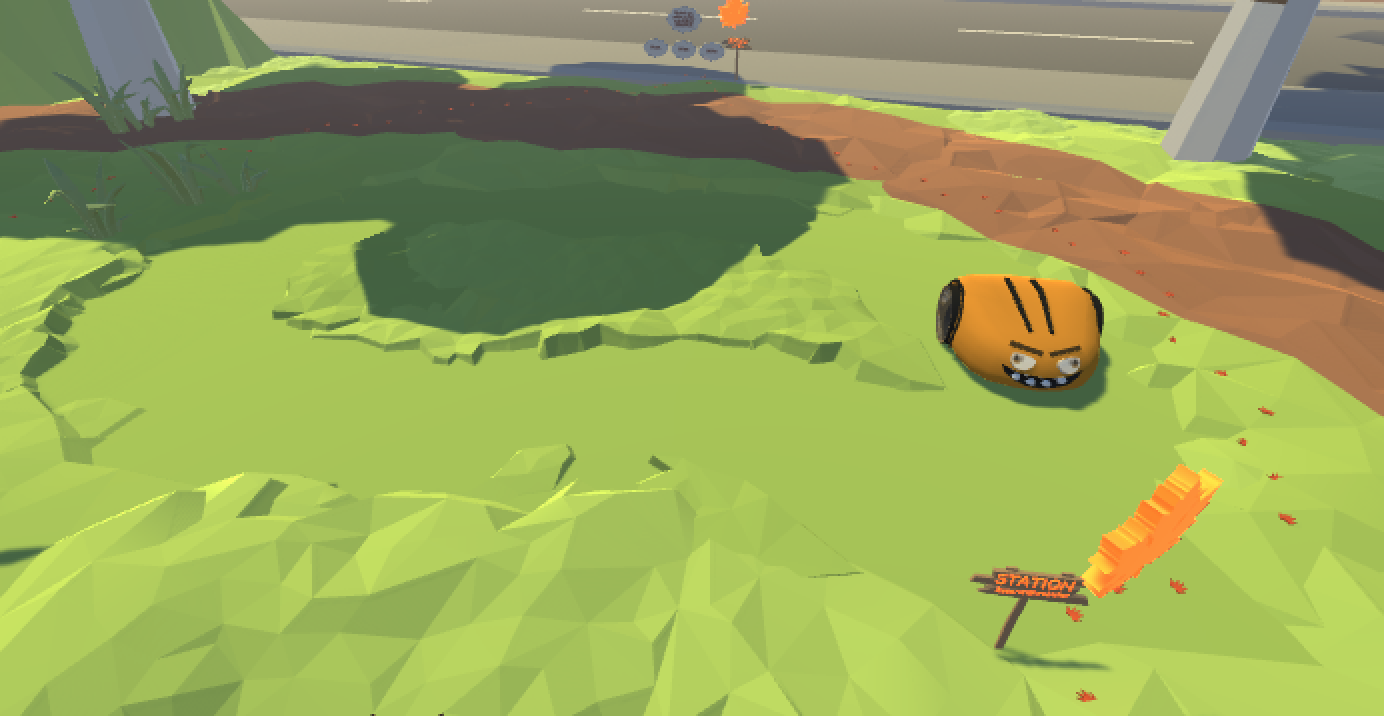
\includegraphics[width=0.675\linewidth]{station_robot.png}
	\caption[Übersicht über die Rasenmäher Station]{Übersicht über die Rasenmäher Station. Quelle: Eigene Aufnahme}
	\label{fig:station_robot}
\end{figure}

In \autoref{fig:station_robot} ist die Übersicht über den Aufbau der Station gegeben. Die Landschaft und der Rasenmäherroboter wurden von Magdalena Bienefeld entworfen. Mithilfe meines Strecken Skripts wurde dem Roboter leben eingehaucht. 

Dazu kann mit den Ankerpunkten 2 und 3 die Streckenform angepasst werden und mit den Ankerpunkten 1 und 4 der Start- und Zielpunkt der Kurve festgelegt werden. Durch aneinanderreihen dieser Kurven fährt der Roboter die geschlossene Kurve ab. Dabei ist zu beachten, dass der Punkt 1 von Kurve A mit dem Punkt 4 von Kurve B und Punkt 4 von Kurve A mit dem Punkt 1 von Kurve B zusammenfallen. Falls dies nicht beachtet wird, kommt es zu Sprüngen in der Strecke. Die Strecke wurde nach dem Vorbild aus einem Video entworfen. \cite{Unity_BezierCurve_Youtube}



\subsection{Problematik}
%Bild einfügen
%Probleme -> ungerade ursp. Fläche --> ging nicht mehr
Einer der ersten Entwürfe der Karte hatte über die gesamte Fläche Unebenheiten. Dies führte allerdings durch die implementierte Gestalt der Bézierkurve dazu, dass der Roboter durch diese Unebenheiten hindurch fährt. 

In ersten Gedanken sollte das Hinzufügen einer Rigidbody Komponente und das Einschalten der Gravitation das Problem beheben. Es sollten die Koordinaten in der xz-Ebene mit der Kurve berechnet werden und der Roboter durch die Gravitation an den Boden gezogen werden. Ein Collider sollte verhindern, dass das Objekt durch die Landschaft fällt. 

Jegliche Versuche führten allerdings nur zu dem Ergebnis, wie es in \autoref{fig:robot_problem} dargestellt ist. Das Problem wurde durch das Anpassen der Landschaft umgangen. Im neuesten Entwurf sieht die abgefahrene Strecke des Roboters nach einer gemähten Wiese aus.

\begin{figure}[H]
	\centering
	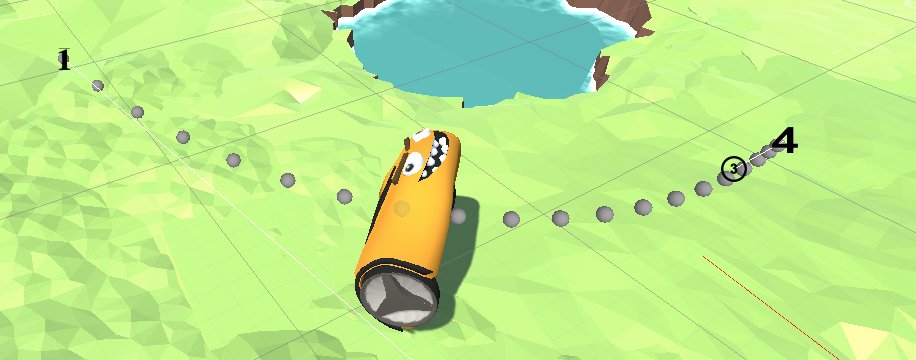
\includegraphics[width=0.5\linewidth]{robot_problem.png}
	\caption[Darstellung des Problems der unebenen Fläche]{Darstellung des Problems der unebenen Fläche. Quelle: Eigene Aufnahme}
	\label{fig:robot_problem}
\end{figure}



\section{Station 8: Straße}
\subsection{Auto Design}
\begin{figure}[H]
	\centering
	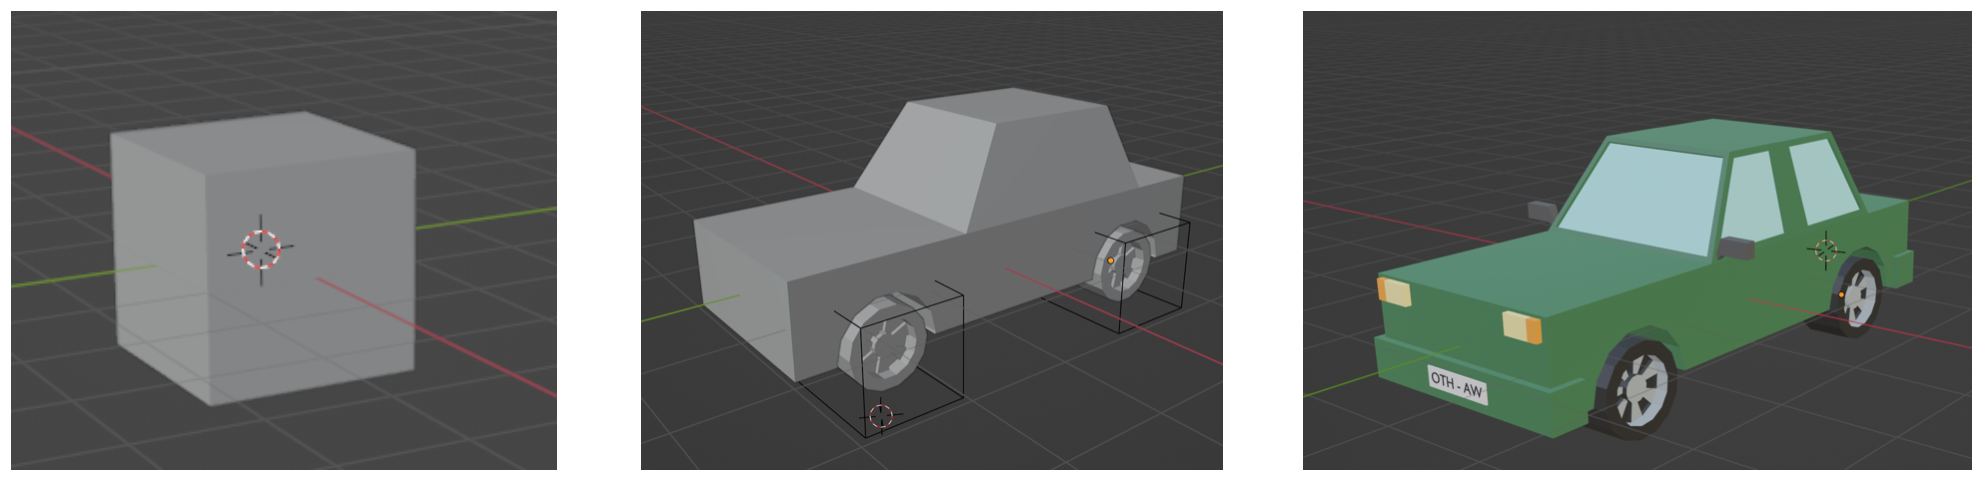
\includegraphics[width=0.8\linewidth]{Development_Car.png}
	\caption[Entwicklungsprozess des Autos mit Blender]{Entwicklungsprozess des Autos mit Blender. Links: Ausgangsobjekt, Mitte: Zwischenstand, Rechts: Fertige Objekt. Quelle: Eigene Aufnahme}
	\label{fig:development_car}
\end{figure}

\begin{figure}[H]
	\centering
	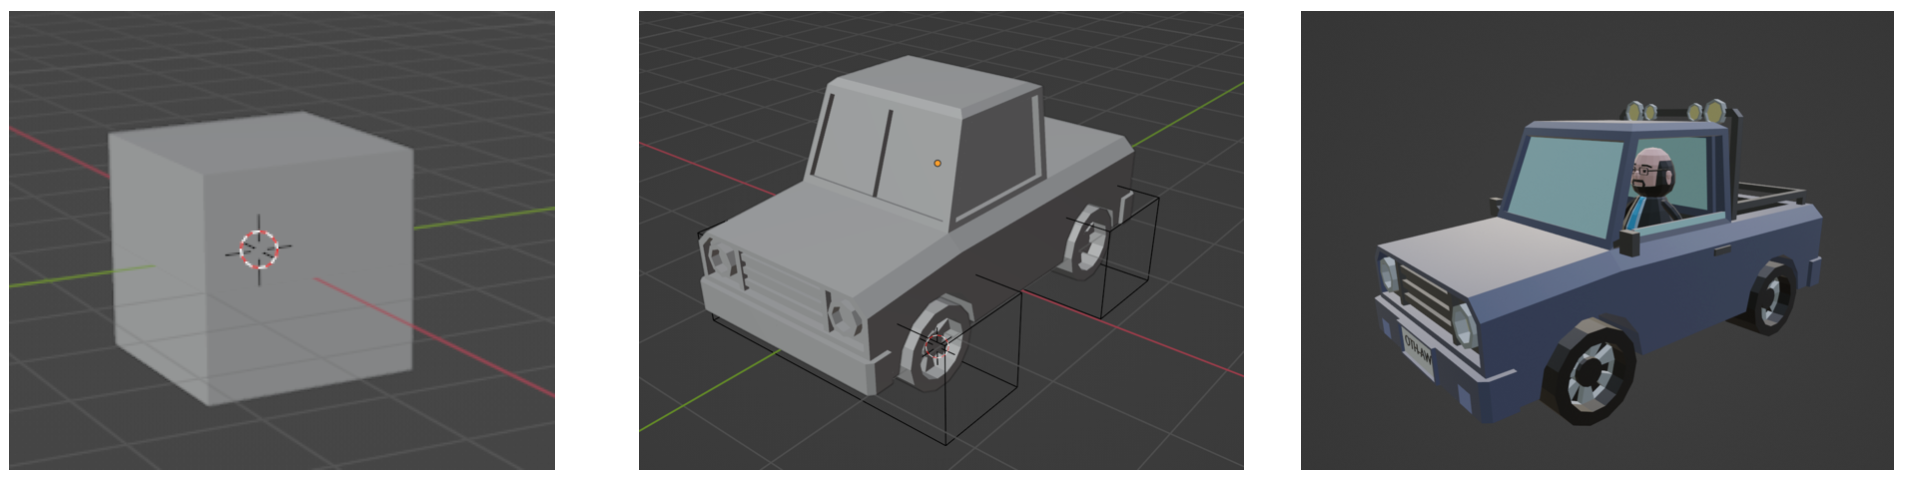
\includegraphics[width=0.8\linewidth]{Development_Pickup.png}
	\caption[Entwicklungsprozess des Pickups mit Blender]{Entwicklungsprozess des Pickups mit Blender. Links: Ausgangsobjekt, Mitte: Zwischenstand, Rechts: Fertige Objekt. Quelle: Eigene Aufnahme}
	\label{fig:development_pickup}
\end{figure}

Mithilfe der 3D-Objektmodellierungssoftware Blender wurden die in \autoref{fig:development_car} und \ref{fig:development_pickup} abgebildeten Objekte erstellt. Ausgehend von dem Würfel sind die Autos Stückweise mit den Werkzeugen (Extrude, Cut, Scale, ...) von Blender erweitert worden. Als Abschluss werden die Materialien für die Texturen der Objekte erstellt.

Im Endprozess kann man mithilfe von Keyframes in Blender die Animationen festlegen. Die Reifen werden mit einer einfachen Rotationsbewegung über eine Zeitspanne verändert. Für die Wink-Bewegung des Charakters im Auto ist auf die Möglichkeiten der Knochen zurückgegriffen worden. Den Körper können eine beliebige Anzahl an Knochen gegeben werden. Diese fungieren wie Gelenke und können anschließend in den Keyframes zu den jeweiligen Zeitpunkten beliebig verändert werden.

\begin{figure}[H]
	\centering
	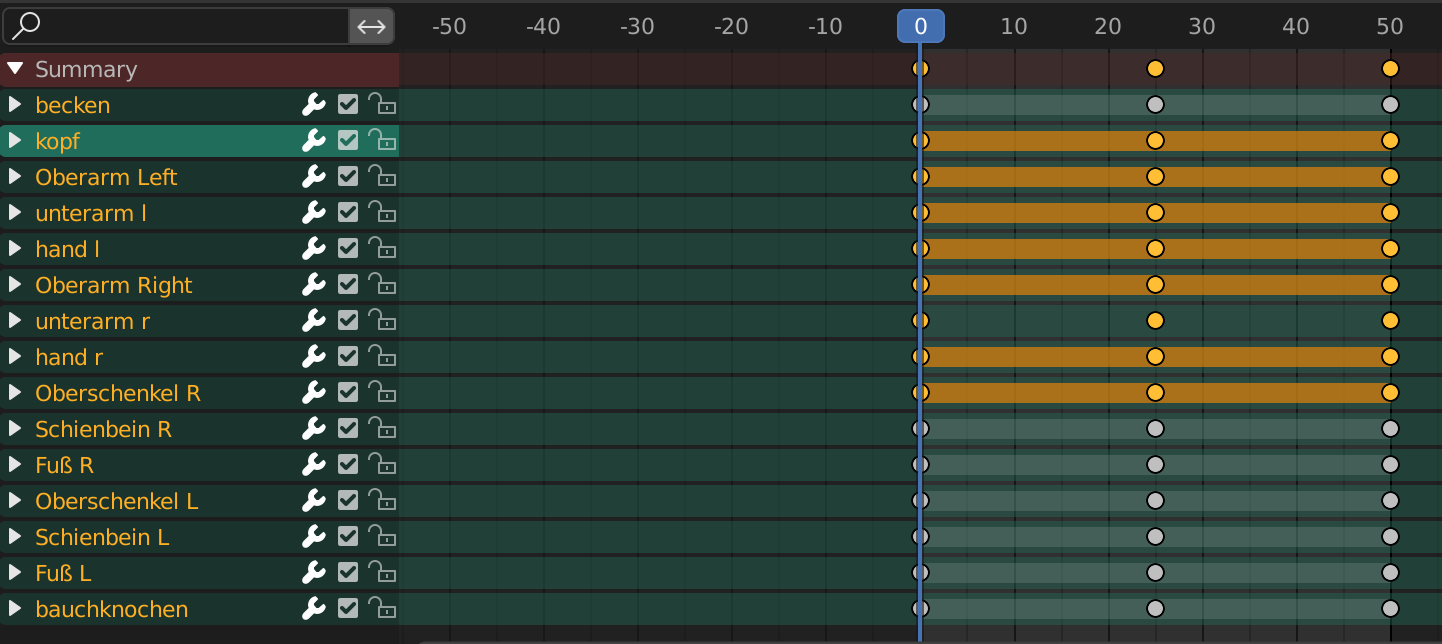
\includegraphics[width=0.5\linewidth]{Keyframes_Animation.png}
	\caption[Keyframes Animation]{Keyframes Animation. Quelle: Eigene Aufnahme}
	\label{fig:keyframes_animation}
\end{figure}

Nach dem Exportieren des fertigen Objekts werden in Unity mithilfe von einem Animator die Animationen abgespielt. Für das gleichzeitige Abspielen der 4 Reifen wurde auf einen Blend-Tree zurückgegriffen. Dieser hat es ermöglicht, dass mit seinen festzulegenden Variablen alle Animationen eines Objektes zur selben Zeit abgespielt werden. 


\subsection{Implementierung}
Beide Autos fahren auf der in \autoref{fig:map} unter Punkt 8 befindlichen Station Straße. Gelangt der Spieler zu dieser Station steht er vor einer Frage und muss diese aus 3 Antwortmöglichkeiten richtig beantworten. Wenn diese erfolgreich beantwortet wird, erhält der Spieler ein weiteres Blatt als Belohnung.

Als kleines Easter-Egg wurde in den Pickup das Asset des Professors Pirkl als Fahrer eingesetzt. Blickt man auf die Straße erkennt man, wie der Fahrer an einem vorbeifährt und dabei aus dem Auto winkt. Das Asset wurde netterweise von Dominik Schweiger zur Verfügung gestellt. Dieser ist angehöriger der Gruppe, die dieses für eine Projektarbeit erstellt haben.


\section{Station 4: Zaun}
Um das Blatt bei dieser Station zu erlangen, muss der Igel der im Zaun feststeckt befreit werden. Dies geschieht, indem der Spieler den Igel mit seinem Controller herauszieht. Für diese 3 unterschiedlichen Zustände existieren 3 Animationen. Abhängig von der Aktion muss eine von diesen ausgeführt werden. Die Schnittstelle zu dem Aufrufen der Aktionen sind in einem Skript implementiert worden. Johannes Horst musste nur noch eine der Funktionen abhängig von seiner ausgeführten Aktion mit dem Controller ausführen.

\section{Spielende}
Für die Registrierung des Spielendes wird ein Event ausgelöst, wenn alle 8 Blätter eingesammelt wurden. Dieses Event triggert eine Funktion und setzt ein Flag auf True. Mithilfe der Basisklasse der Station (Skript von Stefanie Hofmann entwickelt) kann die Position des Spielers abgefragt werden. Wenn dieser sich nach erfolgreichen Beendigen aller Aufgaben im Haus wieder einfindet, ist das Spiel geschafft und die Szene wechselt zu den Credits.




  \chapter{Zusammenfassung und Ausblick}
\section{Zusammenfassung}
Die Entwicklung eines Spiels ist ein komplexer Prozess. Der Entwurf bezieht nicht nur die Implementierung der Logik mit ein, sondern im Laufe der Entwicklung müssen noch weitere Aufgaben bearbeitet werden. Somit musste für das Implementieren der Logik die Programmiersprache C\# erlernt werden. Für das Erstellen der Objekte habe ich einen Einblick in die 3D-Modellierung mit Blender bekommen. Besonders der Entwicklungsprozess der Gegenstände beansprucht abhängig vom Detailgrad der Modellierung ein hohes Maß an Zeit. Durch das Verwenden von Soundeffekten musste man sich zudem noch mit Lizenzen auseinandersetzen.


\section{Ausblick}
Das Spiel lässt sich in vielerlei Hinsicht weiterentwickeln. Zum einen können weiter Stationen implementiert werden, welche das Leben eines Igels noch weiter vertiefen oder die bereits bestehenden Stationen noch verbessert werden. Somit kann die Station des Rasenmähers auf die gesamte Spielwelt ausgeweitet werden und der Roboter mit einem Pathfinding Algorithmus ausgestattet werden. Dieser Algorithmus ermöglicht es den Roboter, unabhängig von der Position des Spielers, jagt auf diesen zu machen. Der Anwender müsste dann auf den Roboter reagieren und sich vor dem Objekt verstecken. Die Station der Straße könnte durch Collider erweitert werden, um einen Aufprall mit dem Igel zu registrieren. Zum erfolgreichen Abschließen der Station müsste es der Spieler auf die gegenüberliegende Seite der Straße schaffen. Daraus könnte sich eine Art Minigame entwickeln, dass den Autos ausgewichen werden muss. Außerdem könnte das Spiel um weitere Level mit anderen Umgebungen erweitert werden. In dem Umfang, dass man sich zum einen in der Stadt zurechtfinden muss und zum anderen auf dem Land.




  %\chapter{Vorlagen}

% Literaturverzeichnis \cite{label}
% Abbildungen, Tabellen, Listing, ... \autoref{label}


\section{Abbildungen}
% small h -> Latex legt fest wo Abbildung am besten liegt wegen Seitenaufteilung
% big H -> Abbildung genau an dieser stelle
\begin{figure}[h]
	\centering
	\includegraphics[width=0.55\linewidth]{sinus_plot.pdf}
	\caption[Beispiel Plot der Matplotlib Bibliothek]{Beispiel Plot der Matplotlib Bibliothek. Quelle: Eigene Aufnahme}
	\label{fig:sinus_plot}
\end{figure}


\section{Tabelle}
% l: linksbündig, c: zentriert, r: rechtsbündig
\begin{table}[H]
	\centering
	\begin{tabular}{l|c|c|c|c|c|c}
		&	Saplte 1	&	Spalte 2	&	Spalte 3	&	Spalte 4	&	Spalte 5	&	Spalte 6\\
		\hline
		Zeile 1		&	1	&	1	&	1 	&	1 &	1	&	1\\
		\hline
		Zeile 2	&	1	&	1	&	1	&	1	&	1		&	1\\
		\hline
		Zeile 3	&  1	&	1	&	1	&	1	&	1	&	1\\
		\hline
		Zeile 4	&	1	&	1	&	1	&	1	&	1	&	1
	\end{tabular}
\end{table}

\section{Programmiercode}
\lstinputlisting[caption=Matplotlib Beispiel Code. Quelle: Eigener Programmcode, label=code_Matplotlib, captionpos=b, firstline=1, lastline=11]{code/Matplotlib_Example.py}

\section{Mathematik}
\subsection{Matrix}
\begin{align}
	M =
	\begin{pmatrix}
		1 &	1	& 1 & 1\\
		1 & 1 & 1 & 1\\
		1 & 1 & 1 & 1\\
		1 & 1 & 1 & 1
	\end{pmatrix}
\end{align}


\subsection{Formel}

\begin{align}
	\begin{split}
		R(\alpha, \beta, \gamma) &=  R_z(\alpha) \cdot R_y(\beta) \cdot R_x(\gamma)\\
		&=\begin{pmatrix}
			C_\alpha\cdot C_\beta & -S_\alpha \cdot C_\gamma + C_\alpha \cdot S_\beta \cdot S_\gamma  & S_\alpha \cdot S_\gamma + C_\alpha \cdot S_\beta \cdot C_\gamma  \\
			S_\alpha\cdot C_\beta & C_\alpha\cdot C_\gamma + S_\alpha\cdot S_\beta\cdot S_\gamma & -C_\alpha\cdot S_\gamma + S_\alpha \cdot S_\beta \cdot C_\gamma \\
			-S_\beta & C_\beta \cdot S_\gamma & C_\beta \cdot C_\gamma
		\end{pmatrix}.
	\end{split}
	\label{EulerToRot}
\end{align}

\begin{equation*}
	[\bar{u}]_x \coloneqq
	\begin{pmatrix}
		0 & -\bar{u}_3 & \bar{u}_2 \\
		\bar{u}_3 & 0 & -\bar{u}_1 \\
		-\bar{u}_2 & \bar{u}_1 & 0 \\
	\end{pmatrix}
\end{equation*}

\begin{align}
	\label{VecToRot1}
	R = I + \sin(\theta)\cdot [\bar{u}]_x + (1-\cos(\theta))\cdot [\bar{u}]_x^2
\end{align}

\section{Aufzählung}
\begin{itemize}
	\item Item 1
	\item Item 2
	\item Item 3
	\item Item 4
\end{itemize}




\section{Station X: Zaun}
\subsection{Animation}
%Skirpt, Animator, Zustände zugreifen

\section{Weiteres}
%Name überlegen für Kapitel
%Animation für Igel Mutter -> von Magdalena -> Blend Tree 



  
 
  % Literaturverzeichnis
  \phantomsection
  \addcontentsline{toc}{chapter}{Literaturverzeichnis}
  \bibliographystyle{natdin}
  \bibliography{literatur}
  \newpage
  
  % Abbildungsverzeichnis
  \phantomsection
  \addcontentsline{toc}{chapter}{Abbildungsverzeichnis}
  \listoffigures
  \newpage

  %Tabellenverzeichnis
  %\phantomsection
  %\addcontentsline{toc}{chapter}{Tabellenverzeichnis}
  %\listoftables
  %\newpage
  
  %Anhang
 %\chapter*{Anhang}

\end{document}    